\documentclass[a4paper, 11pt]{article}
\usepackage{graphicx}
\usepackage{amsmath}
\usepackage[pdftex]{hyperref}

% Lengths and indenting
\setlength{\textwidth}{16.5cm}
\setlength{\marginparwidth}{1.5cm}
\setlength{\parindent}{0cm}
\setlength{\parskip}{0.15cm}
\setlength{\textheight}{22cm}
\setlength{\oddsidemargin}{0cm}
\setlength{\evensidemargin}{\oddsidemargin}
\setlength{\topmargin}{0cm}
\setlength{\headheight}{0cm}
\setlength{\headsep}{0cm}

\renewcommand{\familydefault}{\sfdefault}

\title{Machine Learning 2015: Project 2 - Regression Report}
\author{pungast@student.ethz.ch\\}
\date{\today}

\begin{document}
\maketitle

\section*{Experimental Protocol}
I added nonlinear features to the original features and used a Random Forest classifier to predict the 3 classes.

\section{Tools}
I used Python with scikit-learn 0.17. Source code is attached to the submission.

\section{Algorithm}
I used a Random Forest classifier with 40 trees. Parameters are described below.

\section{Features}
I added the following new features, for each feature x: $log x$, $x log x$, $\sqrt{x}$, $x^3$, $x^4$ and all second-order polynomial combinations of features.

I did not normalise the data because it turned out that neither row-max normalising (dividing all features of each datapoint by the maximum dimension) or column-max normalising (diving all i-th feature values with the maximum i-th feature over all datapoints) improved prediction accuracy in cross-validation.

For visualising the data (for debugging and getting an overview of the data) I used the t-SNE algorithm to map the datapoints into 2 dimensions so that locality information would be conserved. The result is depicted in Figure~\ref{fig:tsne} and shows that the datapoints are quite well linearly separable even in the 2-dimensional space resulting from applying t-SNE.

\begin{figure}[h]
	\begin{center}
	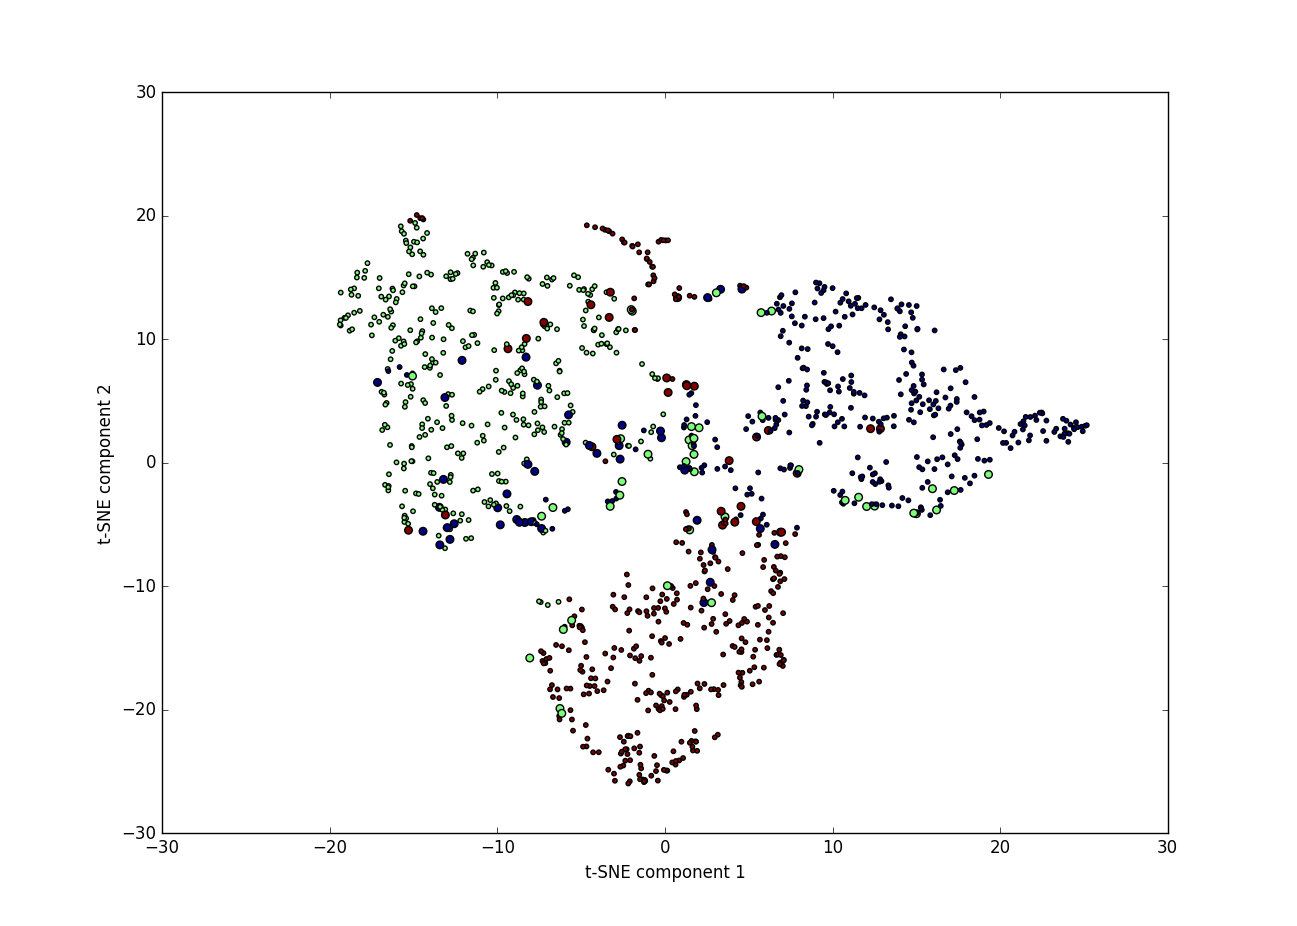
\includegraphics[width=\textwidth]{failures1}
	\end{center}
	\caption{Data after t-SNE transformation into 2 dimensions. Misclassified points are larger than correctly classified points.}
	\label{fig:tsne}
\end{figure}

\section{Parameters}
I used the following parameters, found in 3-fold cross-validation parameter search (in brackets [] are the parameter values I searched over (all combinations)):

\begin{itemize}
	\item Number of trees in forest: 40 [20, 40, 60, 80, 100, 200]
	\item Maximum number of features to consider at each split: 2 [1, 2, 3, 4]
	\item Minimum number of samples required to split an internal node: 5 [1, 3, 5]
\end{itemize}

\section{Lessons Learned}

I also tried SVMs with different kernels (RBF, polynomial, linear) but they were all beat by Random Forest in cross-validated parameter searches. It was a surprise to me that even in a quite extensive parameter sweep, SVMs with all kernels I tried were inferior to Random Forests -- I would have expected SVMs to be able to learn the nonlinearities better.

A hypothesis: the inferiority of SVMs may be caused by the larger sensitivity of SVMs to the lack of normalisation. However, I tested two kinds of normalising for both SVMs and Random Forests and the prediction performance of SVMs still did not improve.

\end{document}
